\documentclass[a4paper, 10pt]{article}
\usepackage[latin1]{inputenc}    % Accept european-encoded (latin1) characters.
\usepackage{a4wide}              % Wide paper
\usepackage[parfill]{parskip}		% skip a line instead of indenting new paragraphs
\usepackage{graphicx}   % For eps figures
\usepackage{epsfig}     % Alternative package
 
\usepackage{fancyhdr} 
\fancyhead[L]{\class \;- \assignment }
\fancyhead[R]{\author }
\renewcommand{\footrulewidth}{0.5pt} % Insert a line above the footer
\pagestyle{fancy}
\usepackage[hang,small,bf]{caption}
\usepackage{palatino}
\usepackage{amsmath}
\usepackage{amssymb}
\usepackage{enumerate}
 
% convenience commands
\renewcommand{\author}{Daniel Standage}
\newcommand{\class}{Stat 430}
\newcommand{\instructor}{Karin Dorman}
\newcommand{\assignment}{HW 3}
\newcommand{\duedate}{September 30, 2010}
 
\newcounter{prob_num}
\setcounter{prob_num}{1}
% usage: \problem
\newcommand{\problem}{\vspace{20pt}\arabic{prob_num}.\stepcounter{prob_num}\par}
% usage: \head{name}{class}{assignment}
\newcommand{\head}{\begin{center}\begin{tabular*}{\linewidth}{l@{\extracolsep{\fill}}r} & \class \;- \assignment \\ & \duedate \end{tabular*}\end{center} \hfill }
% usage: \eqn{equation}{label}
\newcommand{\eqn}[2]{\begin{equation}#1\label{#2}\end{equation}}
 
% begin document
\begin{document}
 
\head
 
%%%%%%%%%%%%%%%%%%%%%%%%%%%%%%%%%%%%%%%%%%%%%%%%%%
\problem

\begin{enumerate}[(a)]
\item There are $3 \cdot 2 = 6$ possible treatments she can apply.
\item The problem states that the selected units are ordered randomly, but it does not say how they are selected from the population. I will assume they were selected randomly from the population of interest. The only other question we can ask is whether the application of treatments is random. My only concern is that the random order of the treatments is recycled. I'm not sure if this is enough to compromise the random nature of treatment application, but if it were up to me, I would consider each unit individually and apply a treatment by random selection of the treatment from a uniform distribution.
\item In this case, the experimental unit is the room.
\item In this case, I would consider each session as a separate room. If there are $m$ rooms and 3 sessions per room, then I would proceed as if there were $3m$ rooms and randomly assign each subject to one of the sessions.
\end{enumerate}

%%%%%%%%%%%%%%%%%%%%%%%%%%%%%%%%%%%%%%%%%%%%%%%%%%
\problem

\begin{enumerate}[(a)]
\item The true $\theta$, as computed below, has a value of 0.1475836.
\begin{verbatim}
> mycauchy <- function(c, location=0, scale=1){
+ return (scale / (pi * ((c - location)^2 + scale^2)))
+ }
> integrate(mycauchy, 2, Inf)
0.1475836 with absolute error < 1.3e-10
>
> 1 - pcauchy(2)
[1] 0.1475836
\end{verbatim}

\item The estimator $\hat{\theta}_1$ can be written as an expectation as follows. \[ P(C > 2) = E[1\{C > 2\}] = \frac{1}{n}\sum_{i=1}^n1\{C > 2\} \] Evaluation of this estimator with Monte Carlo sampling gives $\hat{\theta}_1 = 0.147784$.
\begin{verbatim}
> n <- 1000000
> theta_hat <- sum(rcauchy(n) > 2) / n
> theta_hat
[1] 0.147784
\end{verbatim}

\item Each of the $n$ samples drawn from the Cauchy distribution can be considered a Bernoulli trial, and together they follow a $\textsc{Binom}(n, p)$ where, in this case, $n = 1,000,000$ and $p$ is the probability $\hat{\theta}_1$ of sampling a value greater than 2. Therefore, using the variance of a binomial distribution, we have \[ \textsc{Var}\left(\hat{\theta}_1\right) = \textsc{Var}\left(\frac{1}{n}\sum_{i=1}^{n}1\{C > 2\}\right) = \frac{1}{n^2}\textsc{Var}\left(\sum_{i=1}^{n}1\{C > 2\}\right) = \frac{1}{n^2}\textsc{Var}\left(\textsc{Binom}(n, \hat{\theta}_1)\right) \]\[ = \frac{1}{n^2}np(1-p) = \frac{p(1-p)}{n} = \frac{(0.1475836)(1-0.1475836)}{1,000,000} = 1.26 \cdot 10^{-7} \]
\begin{verbatim}
> p <- 1 - pcauchy(2)
> n <- 1000000
> (1/n)*p*(1-p)
[1] 1.258027e-07
\end{verbatim}

\item The estimator $\hat{\theta_2}$ can be written as an integral as follows. \[ 1-2\theta = 1-2P(C > 2) = 1 - 2 \int_{2}^{\infty}\frac{1}{\pi(c^2+1)}dc \]
This integral cannot be integrated using Monte Carlo integration because of the infinite limit. However, if we recognize the symmetric nature of the Cauchy distribution, we can rewrite the integral as follows. \[ 1 - 2 \int_{2}^{\infty}\frac{1}{\pi(c^2+1)}dc = \int_{-2}^{2}\frac{1}{\pi(c^2+1)}dc \]
This integral can now be approximated using Monte Carlo methods, with $(b-a)\hat{\theta}_2 = 4\hat{\theta}_2 = 0.704701$, or in other words, $\hat{\theta}_2 = 0.1761235$.
\begin{verbatim}
> n <- 1000000
> draws <- rcauchy(n)
> theta_hat_2 <- sum(draws > -2 & draws < 2) / n
> theta_hat_2
[1] 0.704494
> theta_hat_2 / 4
[1] 0.1761235
\end{verbatim}


\item We could use the sample variance $S^2$ to estimate $\textsc{Var}(\hat{\theta}_2)$. Consider the following.
\[ \textsc{Var}(\hat{\theta}_2) = S^2 = \frac{1}{n-1}\sum_{i=1}^{n}(\hat{\theta}_{2i}-\bar{\hat{\theta}}_2)^2 = \frac{1}{n-1}\sum_{i=1}^{n}\left((1-2\hat{\theta}_{1i})-(1-2\bar{\hat{\theta}}_1)\right)^2 \] \[ = \frac{1}{n-1}\sum_{i=1}^{n}\left[2(\bar{\theta}_1 - \theta_{1i})^2\right] = 4\left[\frac{1}{n-1}\sum_{i=1}^{n}(\bar{\theta}_1 - \theta_{1i})^2\right] = 4\textsc{Var}(\theta_1) \]
Therefore the variance for $\hat{\theta}_2$ is four times that of $\hat{\theta}_1$. I would always prefer to choose the estimator with less variance, which in this case is $\hat{\theta}_1$.
\end{enumerate}

%%%%%%%%%%%%%%%%%%%%%%%%%%%%%%%%%%%%%%%%%%%%%%%%%%
\problem

\begin{enumerate}[(a)]
\item
\[ E[\hat{I}(f)] = E\left\{ \frac{1}{n} \sum_{i=1}^{n}\frac{f(X_i)}{g(X_i)} \right\} = \frac{1}{n} \sum_{i=1}^{n}E\left\{ \frac{f(X_i)}{g(X_i)} \right\} = E\left\{ \frac{f(X_i)}{g(X_i)} \right\} \]
\[ = \int X \frac{f(x)}{g(x)}dx = \int_{a}^{b}g(x)\frac{f(x)}{g(x)}dx = \int_{a}^{b}f(x)dx = I(f) \]

\item The variance $\textsc{Var}(\hat{I}(f))$ can be expressed as follows
\[ \textsc{Var}\left(\hat{I}(f)\right) = \textsc{Var}\left(\frac{1}{n}\sum_{i=1}^{n}\frac{f(x)}{g(x)}\right) = \frac{1}{n^2}\sum_{i=1}^{n}\textsc{Var}\left(\frac{f(x)}{g(x)}\right) = \frac{1}{n}\textsc{Var}\left(\frac{f(x)}{g(x)}\right) \]
where
\[ \textsc{Var}\left(\frac{f(x)}{g(x)}\right) = E_g\left[\left(\frac{f(x)}{g(x)}-E_g\left[\frac{f(x)}{g(x)}\right]\right)^2\right] = E_g\left[\left(\frac{f(x)}{g(x)}\right)^2\right]-\left(E\left[\frac{f(x)}{g(x)}\right]\right)^2 \]\[ = \int_{a}^{b}\left[\left(\frac{f(x)}{g(x)}\right)^2g(x) - \left(E\left[\frac{f(x)}{g(x)}\right]\right)^2\right]dx = \int_{a}^{b}\left[\frac{f^2(x)}{g(x)} - \left(E\left[\frac{f(x)}{g(x)}\right]\right)^2\right]dx \]
%where \[ {Var}\left(\frac{f(x)}{g(x)}\right) = \int_{a}^{b}\left[\frac{f(x)}{g(x)}-E\left[\frac{f(x)}{g(x)}\right]\right]^2 \]
Therefore, if we let $a = 0, b=1, f(x) = \frac{1}{b-a} = 1,$ and $ g(x) = x$, then $\textsc{Var}\left(\hat{I}(f)\right)$ is infinite. On the other hand, if we let $a = 0, b=1, f(x) = x^3 = 1,$ and $ g(x) = x$, then $\textsc{Var}\left(\hat{I}(f)\right)$ is finite.

\item If $g(x) \sim \textsc{Unif(0,1)}$, then we have
\[ \hat{I}(f) = \frac{1}{n}\sum_{i=1}^{n}f(x) = \int_{0}^{1}f(x)dx \]
\end{enumerate}

%%%%%%%%%%%%%%%%%%%%%%%%%%%%%%%%%%%%%%%%%%%%%%%%%%
\problem

Since $X_i, ..., X_n \sim \textsc{Norm}(\mu_X, \sigma^2)$, we know that \[ \frac{n-1}{\sigma^2}S_X^2 \sim \chi^2_{n-1} \] Likewise, we have \[ \frac{m-1}{\sigma^2}S_Y^2 \sim \chi^2_{m-1} \] The $F$ distribution is perfect for modeling quotients of $\chi^2$ distributions. In this case, we have \[ \frac{S_X^2}{S_Y^2}\cdot \frac{m-1}{n-1} \sim F(n-1, m-1) \]
The hypothesis being tested is \[ H_0: S_X^2 = S_Y^2 \]

%%%%%%%%%%%%%%%%%%%%%%%%%%%%%%%%%%%%%%%%%%%%%%%%%%
\problem

\begin{enumerate}[(a)]
\item I first calculated the sample mean $\bar{Y}$ and the sample standard deviation $S$. I then plotted a histogram of the sample and plotted a normal distribution ($\textsc{Norm}(\bar{Y}, S^2)$) over that histogram. I then adjusted the standard deviation until I was visually satisfied with the fit. Using this method, I calculated $\bar{Y} \approx 0.00126, S \approx 0.01998$, and it appears that $Y \sim \textsc{Norm}(\bar{Y}, 0.0135^2)$.

\begin{center}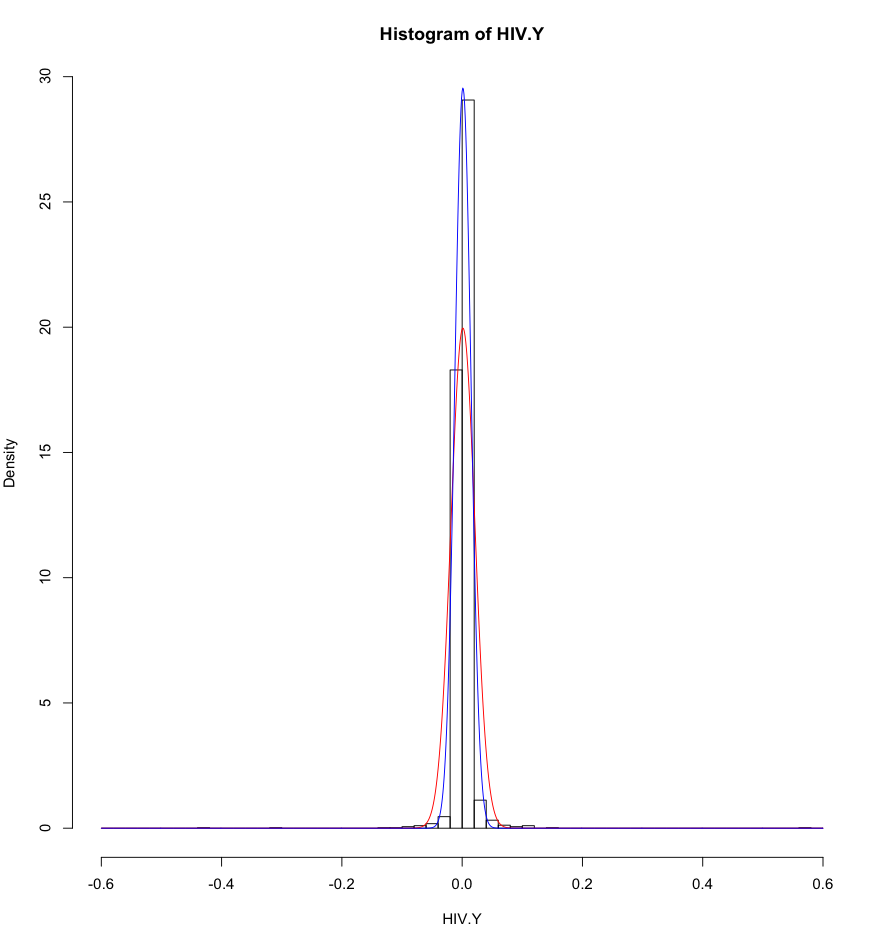
\includegraphics[scale=0.3]{hiv_y.png}\end{center}

\begin{verbatim}
> hiv <- read.table("hiv_status_data.Rtxt")
> y_bar <- mean(hiv$Y)
> y_bar
[1] 0.001258547
> S <- sd(hiv$Y)
> S
[1] 0.01998172
> hist(hiv$Y, breaks=seq(-.6, .6, .02), freq=F, xlab="HIV.Y",
+ main="Histogram of HIV.Y")
> x <- seq(-.6, .6, .001)
> y <- dnorm(x, y_bar, S)
> lines(x, y, type="l", col="red")
> y <- dnorm(x, y_bar, .0135)
> lines(x, y, type="l", col="blue")
\end{verbatim}

\item Assuming $Y \sim \textsc{Norm}(\bar{Y}, 0.0135^2)$, the expected value of $Y$ is the sample mean $\bar{Y} \approx 0.00126$.
\item The interval $[.00048, .00204]$ provides a 95\% confidence interval for the population expected improvement rate.
\begin{verbatim}
> Y.bar <- mean(hiv$Y)
> S <- sd(hiv$Y)
> q <- qnorm(.975)
> dim(hiv)
[1] 2501   39
> n <- 2501
> Y.bar - q*(S/sqrt(n))
[1] 0.0004754349
> Y.bar + q*(S/sqrt(n))
[1] 0.002041659
\end{verbatim}

\item Because the p-value $p = 0.4$ of this $t$-test is greater than any reasonable choice of $\alpha$, we cannot reject the null hypothesis that that there is no difference between the outcomes for patients from the two clinics.

\begin{verbatim}
> y.clinic1 <- subset(hiv, Clinic.ID == 1, select=c("Y"))
> y.clinic2 <- subset(hiv, Clinic.ID == 2, select=c("Y"))
> t.test(y.clinic1, y.clinic2)

        Welch Two Sample t-test

data:  y.clinic1 and y.clinic2 
t = 0.8419, df = 1743.661, p-value = 0.4000
alternative hypothesis: true difference in means is not equal to 0 
95 percent confidence interval:
 -0.0009123599  0.0022847071 
sample estimates:
   mean of x    mean of y 
0.0016124712 0.0009262976
\end{verbatim}

\item Because the p-value $p = 0.01273$ of this 1-tailed 	$t$-test is less than $\alpha = 0.05$, we can safely reject the null hypothesis that there is no improvement in outcome for patients with drug treatments versus patients without drug treatments.
\begin{verbatim}
> drugs <- c("amprenavir", "atazanavir", "darunavir",
+ "fosamprenavir", "indinavir", "lopinavir", "nelfinavir",
+ "ritonavir", "saquinavir", "tipranavir")
> hiv.d <- hiv[, c("Patient.ID", "Y", drugs)]
> hiv.d$numRx <- rowSums(hiv.d[, drugs])
> y.no.drug <- hiv.d$Y[hiv.d$numRx == 0]
> y.with.drug <- hiv.d$Y[hiv.d$numRx > 0]
> t.test(y.with.drug, y.no.drug, alternative="g")

        Welch Two Sample t-test

data:  y.with.drug and y.no.drug 
t = 2.2359, df = 2146.263, p-value = 0.01273
alternative hypothesis: true difference in means is greater than 0 
95 percent confidence interval:
 0.0004660495          Inf 
sample estimates:
   mean of x    mean of y 
0.0018887881 0.0001236902 

\end{verbatim}

\item Because the p-value $p = 0.1333$ of this paired $t$-test is greater than $\alpha = 0.05$, we cannot reject the null hypothesis that there is no affect when adding a protease inhibitor treatment following a treatment without protease inhibitor.

\begin{verbatim}
> # Find patients with multiple Y values
> list.no.drug <- subset(hiv.d, numRx == 0, select=c("Patient.ID", "Y"))
> list.with.drug <- subset(hiv.d, numRx > 0, select=c("Patient.ID", "Y"))
> repeated.ids <- intersect(list.no.drug$Patient.ID, list.with.drug$Patient.ID)
>
> # Separate the Y values based on number of treatments, average multiples
> patients.no.drug = subset(list.no.drug, Patient.ID %in% repeated.ids,
+ select=c("Patient.ID", "Y"))
> patients.with.drug = subset(list.with.drug, Patient.ID %in% repeated.ids,
+ select=c("Patient.ID", "Y"))
> y.no.PI = aggregate(patients.no.drug, list(patients.no.drug$Patient.ID),
+ mean)$Y
> y.with.PI = aggregate(patients.with.drug,
+ list(patients.with.drug$Patient.ID), mean)$Y
>
> # Perform t-test
> t.test(y.with.PI, y.no.PI, paired=T)

        Paired t-test

data:  y.with.PI and y.no.PI 
t = 1.5071, df = 210, p-value = 0.1333
alternative hypothesis: true difference in means is not equal to 0 
95 percent confidence interval:
 -0.001076692  0.008066891 
sample estimates:
mean of the differences 
            0.003495099
\end{verbatim}

\end{enumerate}

\end{document}